\chapter{LHC and the CMS experiment}
\label{chap:chapter_3}
A brief introduction to the collider LHC \ref{sec:lhc} and the experiment CMS \ref{sec:cms} is provided, along with technical information. In section \ref{sec:HL-LHC} the High-Luminosity LHC upgrade is discussed, with a particular focus on its physics program and the study of the Higgs self-coupling.

\section{LHC}
\label{sec:lhc}
The Large Hadron Collider (LHC) is the largest and most powerful particle collider constructed so far, located near Geneva, Switzerland, and built by the European Organization for Nuclear Research (CERN).  

The LHC is located underground, and it uses the tunnel of a previous collider, the Large Electron-Positron Collider (LEP), a ring of about 27 km in circumference and situated over 100 metres underground.

The LEP was active from 1989 to 2000 and collided electrons and positrons with centre of mass energy of $\sqrt{s} = 91$ GeV up to 200 GeV in the later stages of the project.  

Notable results obtained from LEP are the discovery of Z and $W^{\pm}$ bosons, and the estimation of the number of light neutrinos.

The LHC started its collision in 2010, and it was constructed to probe the physics of the SM and beyond, in particular to search for the Higgs boson, discovered in 2012.

It relies on a complex structure of accelerators to provide beams of protons currently colliding at centre of mass energy of $\sqrt{s} = 13.6$ TeV.

\subsubsection{Technical characteristics}

The main idea around which revolves LHC (and previously LEP) is the concept of the synchrotron, an accelerating technique in which the accelerated particles travel around a fixed circular path.\\
To obtain this, the magnetic field that bends the trajectory is increased with time to keep it synchronized with them, hence the name.\\
Obviously, because of the very high energies provided to the particles (6.5 TeV per proton), one synchrotron is not enough, and that is why CERN is a complex structure of accelerators and storage rings, as can be seen in fig. \ref{cern_complex}.
\begin{figure}
    \centering\includegraphics[width=\textwidth]{images/CERN_accelerator_complex.jpg}
    \caption{CERN accelerator complex, with the position of the various experiments highlighted as well}
    \label{cern_complex}
\end{figure}

Discussing specifically the LHC collider, as already stated, it consists of an underground tunnel of 26.7 km. The choice of an underground facility was made for economical convenience, and also to have the natural shielding of the Earth's crust against background radiation.\\
The tunnel contains two beam pipes in which the particles travel in opposite directions, and which intersect at four different points, where the four main experiments are located, allowing the particle collisions. The trajectory of the particles is ensured by 1232 dipole magnets, and an additional 392 quadrupole magnets are used to keep the beams focused, with particular attention around the interaction points.\\ 
All the magnets, made of copper-clad niobium-titanium, are superconducting magnets, and operate at the temperature of 1.9 K (-271.25 $^{\circ}$C), which is provided with the use of superfluid helium-4. In this way, a magnetic field of up to 8.3 T is obtained.\\
To have better control over the acceleration and collisions, the beams are not continuous, rather the protons are bunched together in bunches long about 8 cm. In this way, collisions happen every 25 ns, and this leads to a bunch collision rate of 40 MHz.\\
The bunches are accelerated using radiofrequency cavities, where the electromagnetic field oscillates at a tuned frequency, delivering energy to the protons.
Radiofrequency cavities are also extremely useful in keeping the bunches compact because, when the beam has reached its maximum energy, an ideally timed proton won't be further accelerated, while, if the timing of the proton is slightly different from the tuning, it will be accelerated (delayed) or decelerated (anticipated), guaranteeing the desired energy to each proton and the keeping of the bunch structure.  
\subsubsection{Luminosity}
The luminosity is defined as the ratio between the rate of events of a considered process and the cross-section of that process:
\begin{equation}
    L = \frac{R}{\sigma} \quad [cm^{-2}s^{-1}]
\end{equation}
In the specific case of a circular accelerator, with the assumption of Gaussian profiles in all dimensions, and assuming equal beams in both directions, we can define the instantaneous luminosity as:
\begin{equation}
    L = \dfrac{N_1N_2N_b f}{4\pi\sigma_x\sigma_y},
    \label{luminosity}
\end{equation}
where $N_1 \text{and} N_2$ are the particles in the two beams, $N_b$ is the number of bunches, $f$ is the frequency of interaction, and $\sigma_x \text{and} \sigma_y$ are the bunch lengths over the two directions.\\
The average peak luminosity provided from LHC during the Run2 has been of $L =  2.1 \cdot 10^{34} cm^{-2}s^{-1}$, doubling the value from Run1, of {}.\\ 
However, this level of luminosity brings a disadvantage, that is, the presence of pile-up collisions. \\
Pile-up collisions indicate the number of additional proton-proton collisions that happen in the same bunch, and that generate background noise. To make an example, during Run2, the average pile-up collisions amounted to  
Integrating \ref{luminosity} over time, we find the integrated luminosity, which is the total number of collisions produced over a period of time.\\
A plot of the integrated luminosity over time and up to 2018 is reported in plot \ref{luminosity}
\begin{figure}
    \centering
    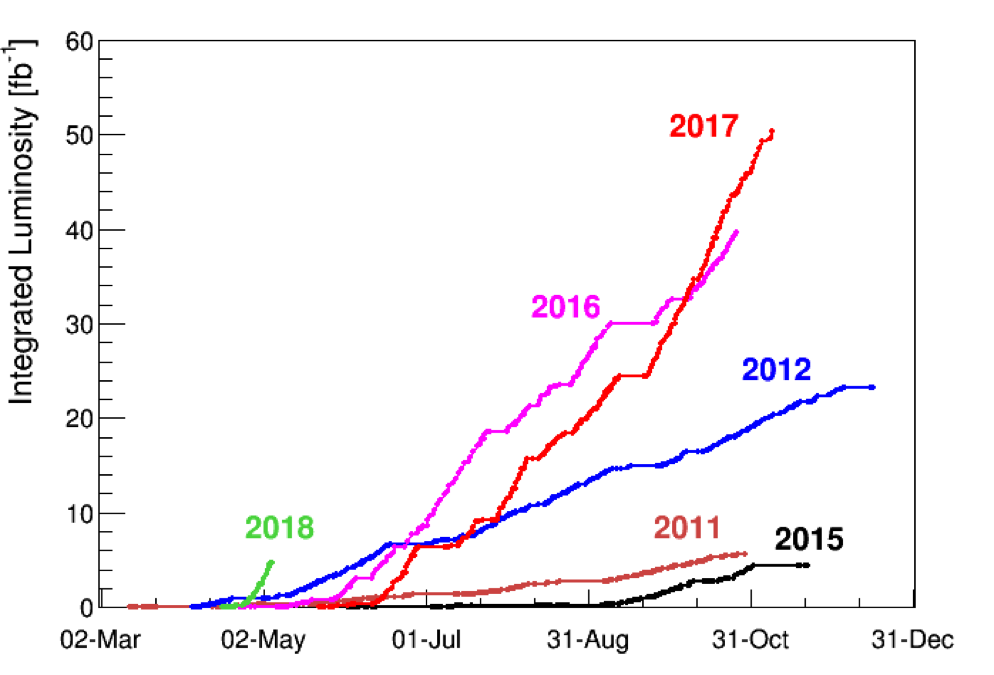
\includegraphics[width= \textwidth]{images/luminosity.png}
    \caption{Integrated luminosity over time}
    \label{luminosity}
\end{figure}
Integrated luminosity is a crucial parameter to take into account because most of the studied processes are rare, and statistics is needed.\\
\subsubsection{Reference frame}
We consider a right-handed coordinate system, where the z axis is parallel to the beam direction.\\
We then define the azimuthal angle $\phi$ as the angle in the xy plane, and the polar angle $\theta$ in the z direction.\\
The typical kinematic variables for the particles are:
\begin{itemize}
    \item $p_T$: the transverse momentum, defined as the amount of momentum perpendicular to the beam direction;
    \item $\phi$;
    \item $m$: the invariant mass of the particle;
    \item $\eta$: the pseudorapidity, defined as 
    \begin{equation*}
        \eta = \frac{1}{2}\ln(\frac{|p|+ p_z}{|p| - p_z}) = - \ln(\tan\frac{\theta}{2})
    \end{equation*}
    is another way to indicate the angle of the particle with the z axis; it is 0 if the particle is perpendicular to the beam direction, and it's greater the more the particle is aligned to the beam direction.
\end{itemize}
\section{CMS}
\label{sec:cms}
The Compact Muon Solenoid (CMS) is one of the main experiments at LHC. It's a general-purpose experiment, that is, it was designed to be able to observe any phenomena the LHC might reveal.\\
It is 15 metres high and 21 metres long, and it weighs 14000 tons.\\
A schematic summary of the overall structure of the detector is reported in fig. \ref{cms}.\\
Further reading on the original project can be found at Ref. \cite{cms_detector}
\begin{figure}
    \centering
    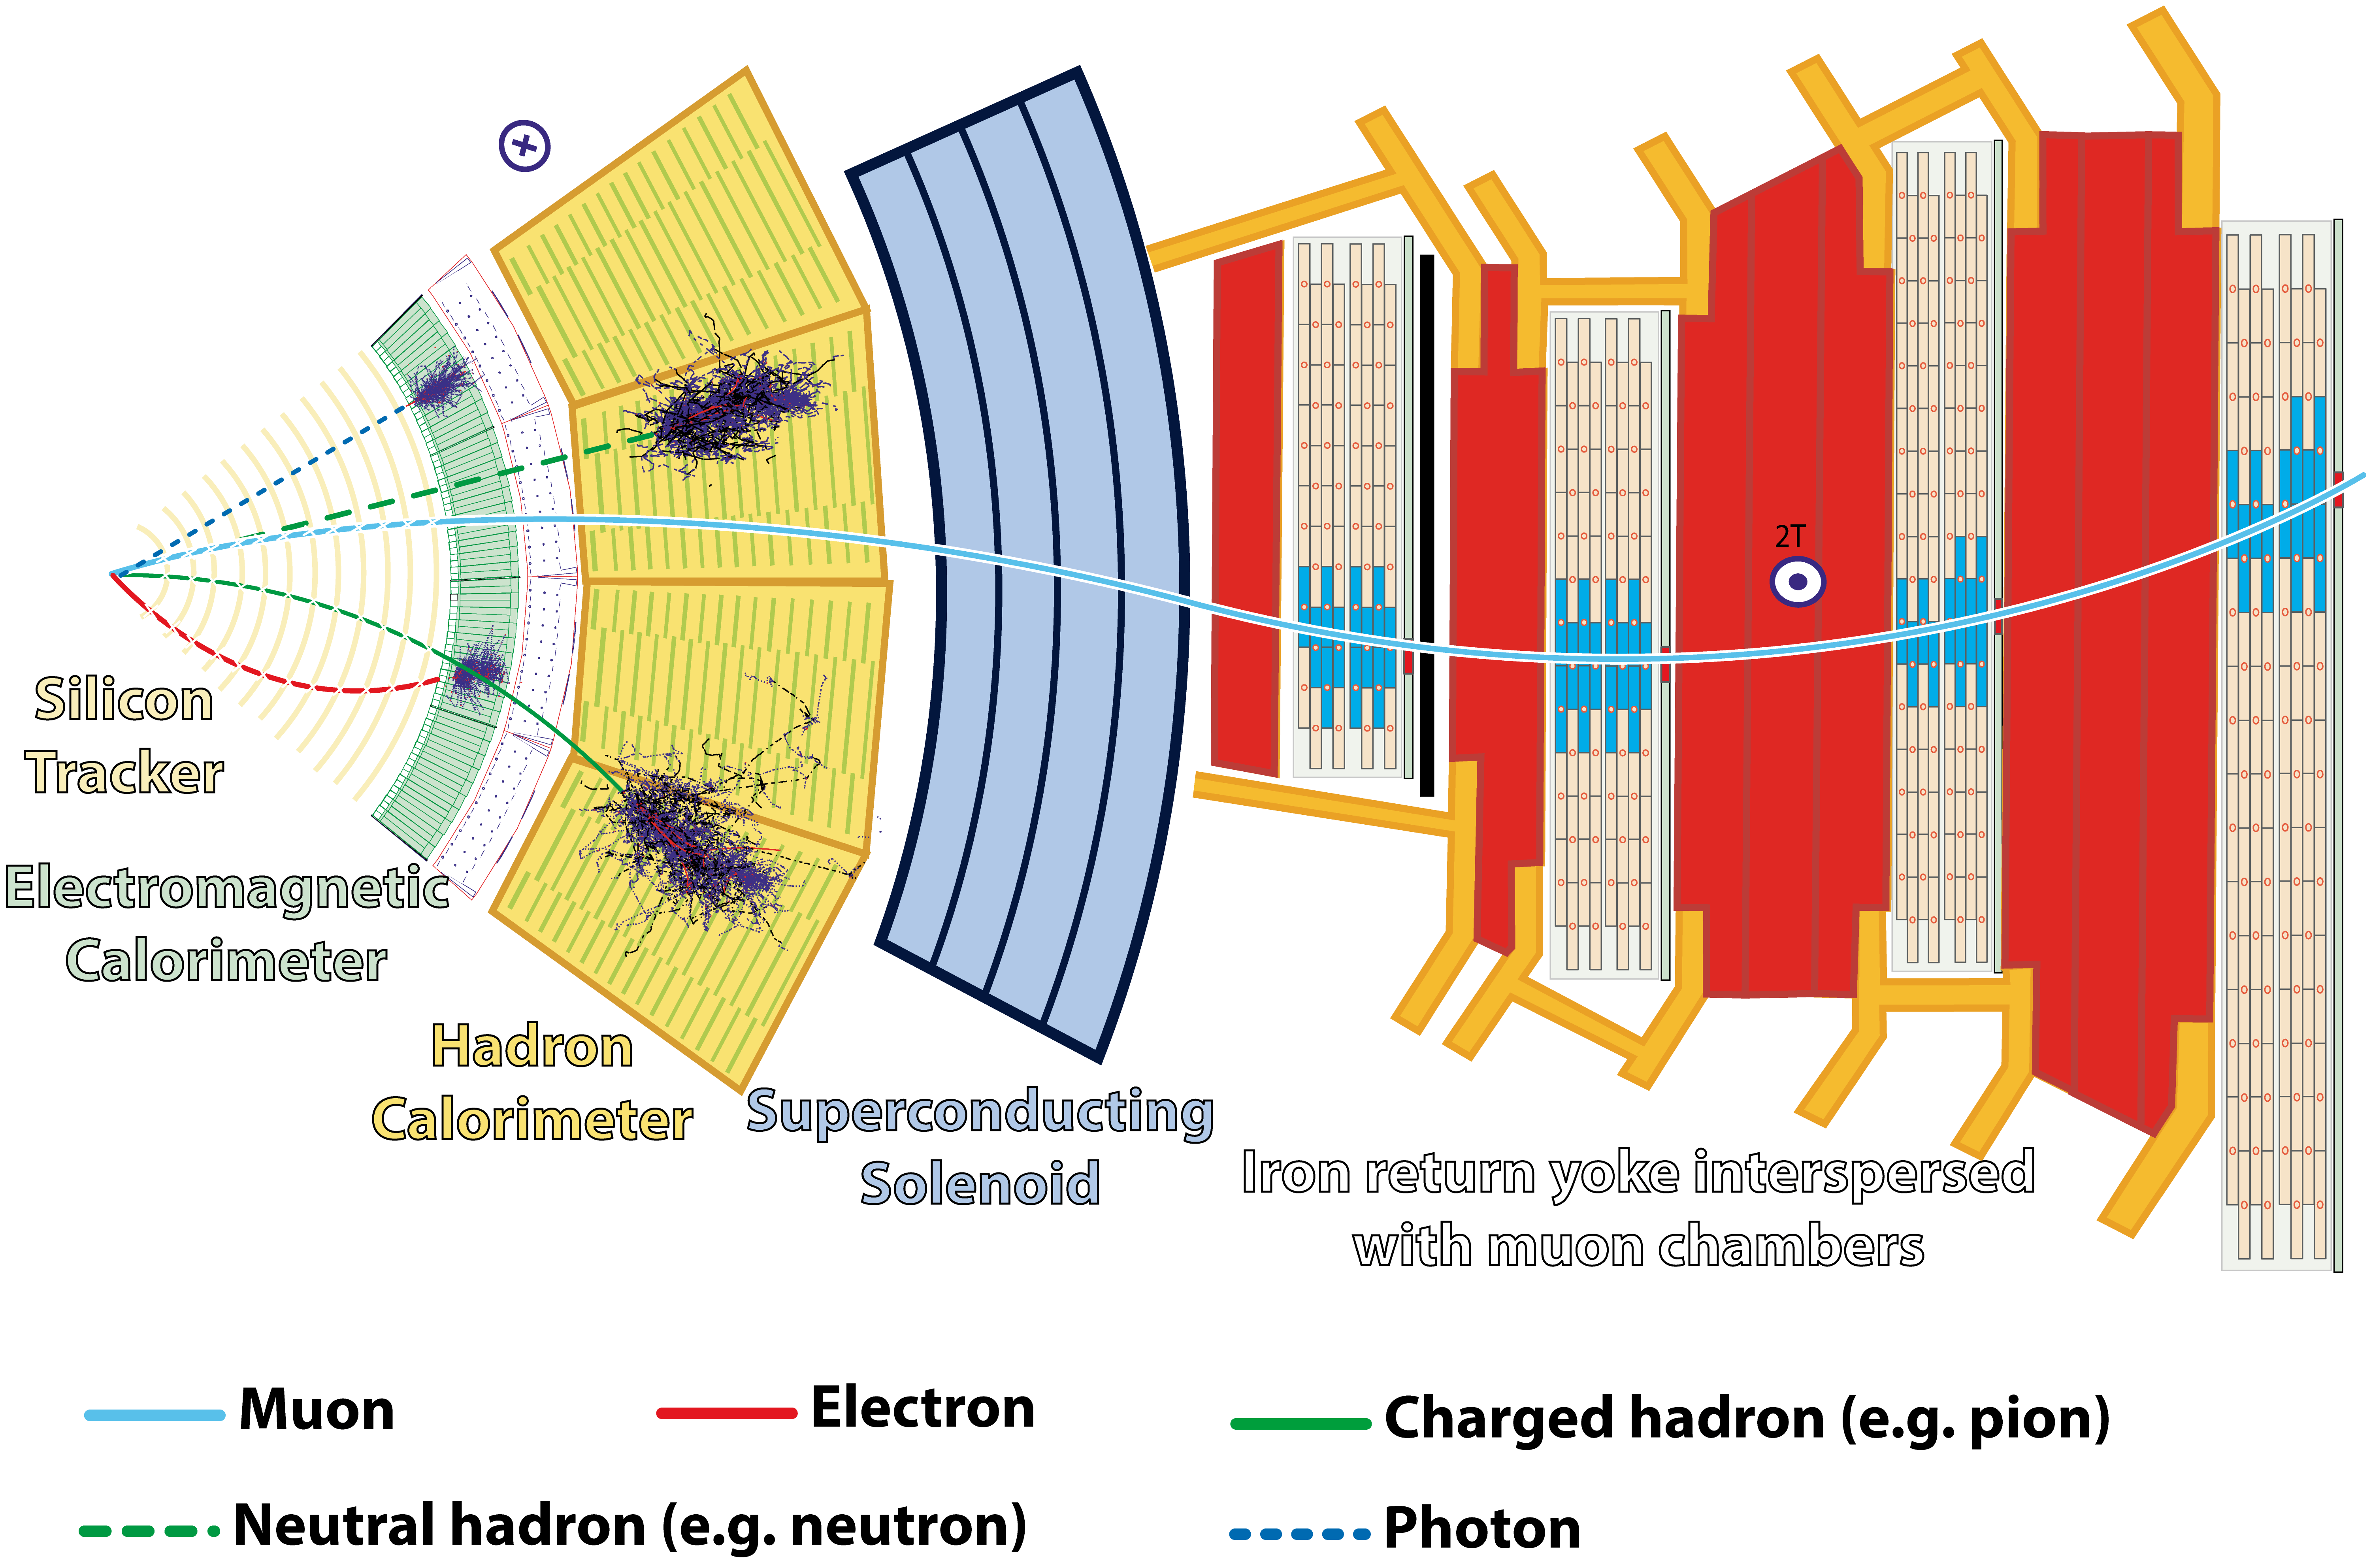
\includegraphics[width = \textwidth]{images/cms.png}
    \caption{Schematic structure of the CMS experiment}
    \label{cms}
\end{figure}
\subsection{Tracker}
Starting from the interaction point, the particles go through the tracker. This section is designed to have precise measurements of the tracks of charged particles and the primary interaction vertices.\\
The tracks are bent using the homogeneous magnetic field of 3.8 T, and the actual revelation is made with the silicon pixel detector in the innermost section, and with silicon microstrip after; overall, the tracker has a diameter of 2.5 m.\\
Pixel detectors are used to ensure high granularity, due to the huge number of tracks present.
This part of the apparatus is the one that withstands the highest amount of radiation.\\
The acceptance of the tracker is of $|\eta|<2.5$.\\
In the forward regions, two disks are present, one at each end, to improve impact parameter measurements and provide points with sufficient resolution for reconstructing secondary vertices from decays of particles containing \emph{c} or \emph{b} quarks.
\subsection{Calorimeters}
Outside the tracker, the electromagnetic calorimeter (ECAL) and then the hadronic calorimeter (HCAL) are located.\\
Calorimeters are used to absorb and measure the energy of all incoming particles (except for neutrinos, which essentially don't interact). \\
When high-energy particles traverse a dense medium, they produce secondary particles with lower energies due to the phenomenon called particle showering. The characteristics of these showers depend on the type of particle.\\
\textit{Electromagnetic showers} are produced by particles that interact mainly electromagnetically, such as electrons, positrons, and photons. Their length is related to the radiation length $X_0$ \footnote{Radiation length: mean length inside the material at which the energy of an electron is reduced due to bremsstrahlung by a factor $e^{-1}$; it's characteristic of a material.} of the material with the following formula:
\begin{equation}
    X = X_0 \frac{\ln(E_0/E_c)}{\ln 2},    
\end{equation}
where $E_0$ is the initial energy of the particle and $E_c$ is the critical energy \footnote{Critical energy: energy at which the bremsstrahlung rate coincides with the collision loss rate (for ionization and excitation)}.
So, to completely absorb the energy from the incoming particles, the calorimeters are designed to have a width equal to 2–3 times $X_0$. %numeri che vanno ricontrollati\\
\textit{Hadronic showers} are produced by particles that interact mostly strongly because of processes like hadron production, nuclear deexcitation and pion decay. This type of shower takes longer to develop, and its length scales with the nuclear interaction length:
\begin{equation}
    \lambda = \frac{A}{N_A \sigma_{abs}},
\end{equation}
where A is the mass number, $N_A$ is the Avogadro number and $\sigma_{abs}$ is the absorption cross-section.
\\
As a trivial example, we report the radiation length and interaction length for different materials in table \ref{x_0}.
\begin{table}[h]
\centering
    \begin{tabular}{c|c|c}
 Elements &$X_0 [g cm^{-2}]$ & $\lambda [g cm^{-2}]$ \\\hline
     H$_2$ &  61.28 & 50.8 \\\hline
     Si & 21.82 & 106.0\\\hline
     Fe & 13.84 & 131.9\\\hline
     Pb & 6.37 & 194 \\
    \end{tabular}
    \caption{Summary of radiation length and interaction length for some elements}
    \label{x_0}
\end{table}

Calorimeters need to be as precise as possible to detect the presence of missing energy, that is, the energy carried by particles that don't interact with the medium, like neutrinos or BSM particles, and that appear as energy that disappears during the event.
\subsubsection{ECAL}
The ECAL is a hermetic homogenous \footnote{homogenous vs sample tbw} calorimeter made of lead tungstate crystals (PbWO$_4$); it is used to measure the energy of the electromagnetic showers with the use of photodiodes and phototriodes.\\
Two parts of the ECAL can be distinguished: the barrel section, with pseudorapidity coverage of up to $|\eta|= 1.48$, and the endcaps, which extend the coverage up to $|\eta| = 3.0$.
The use of PbWO$_4$ is innovative, and it leads to the possibility of having a fast calorimeter due to the short scintillation decay time\footnote{Scintillation decay time: time required for scintillation emission light to decrease to $e^{-1}$ of its maximum} and with fine granularity, thanks to their high density and short radiation length ($X_0$ = 0.89 cm), which is important for the energy resolutions.\\
One of the driving criteria was to be able to detect the $H\longrightarrow\gamma\gamma$ decay.\\
To have further spatial precision, the endcaps also have a preshower detector within the region $1.653 < |\eta|< 2.6$, which is used to discriminate between a highly energetic photon and a pair of low-energy photons coming from the decay of short-lived particles like neutral pions. The preshower detector is made of a layer of lead and then of silicon; when a photon passes through, it makes an electromagnetic shower that is detected by the silicon sensors, and from which the energy of the photon is measured, leading to the discrimination.\\
Fig. \ref{ecal} shows a schematic representation of the ECAL.
\begin{figure}[h]
    \centering
    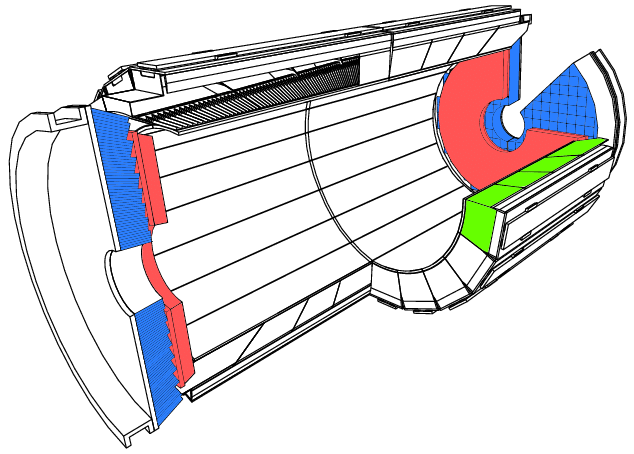
\includegraphics[width = 0.6\textwidth]{images/ecal.png}
    \caption{Schematic representation of the ECAL. In green the barrel, in blue the endcaps and in red the preshowers.}
    \label{ecal}
\end{figure}
\subsubsection{HCAL}
HCAL is a sampling calorimeter: there is an absorber made of steel and brass ($\lambda = 16.42 cm $) that slows the particles down, and plastic scintillators (with thickness that goes from 40 up to 75 mm) that measure the energy of the hadronic showers.\\
To guarantee the maximum pseudorapidity coverage, HCAL is composed of four parts:
\begin{itemize}
    \item the barrel (HB): it covers up to $|\eta| 1.3$, and its coverage in interaction lengths goes from 5.82$\lambda$ up to  10.6 $\lambda$, to which it must be added 1.1 $\lambda$ given by the ECAL.
    \item the endcap (HE): it covers the region 1.3 $<|\eta| < 3$ and contains about 34\% of the particles produced in the final state. This means that the HE needs high radiation tolerance, especially for $\eta\approx$3. Its coverage in interaction lengths is about 10$\lambda$.
    \item the outer calorimeter (HO): it's located outside the solenoid that surrounds HB, and it covers the central region in pseudorapidity (so up to $|\eta| 1.3$) to provide better containment for hadron showers, in particular late starting showers. It extends the coverage in interaction lengths of the HB to at least 11.8 $\lambda$.
    \item the Forward calorimeter (HF): it covers the region of highest pseudorapidity, where the particle fluxes are highest. This means the HF will need to be highly radiation resistant, which is why quartz fibres were chosen as active medium. However, because it exploits Cherenkov radiation for detection, it's mostly sensitive to electromagnetic showers, while it is practically insensitive to neutrons.
\end{itemize}

Fig. \ref{hcal} summarises the various components of HCAL.
\begin{figure}[ht]
    \centering
    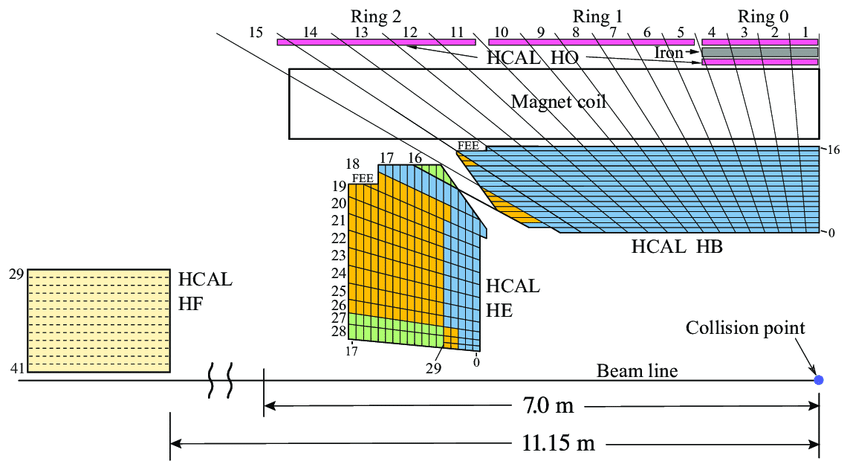
\includegraphics[width = 0.8\linewidth]{images/hcal.png}
    \caption{Schematic representation of a quarter of HCAL}
    \label{hcal}
\end{figure}
\subsection{Muon system}
Muons are a very useful tool that can be used to recognize signatures of interesting processes above the high background rate present. An example of process would be the decay $H\rightarrow ZZ\rightarrow 4 l$, where the two Z decay into charged leptons (the \textit{golden channel}). The case where the leptons are muons is the cleanest one, because the electrons interact with matter inside the detector, while muons are not affected as much.\\
The muon system has three functions: muon identification, momentum measurement, and triggering. \\
It is located inside the returning yoke of the magnetic solenoid, which is used as a hadron absorber as well as to bend the muons and study the momentum from its tracks; between the plates of the yoke, the particle detectors are set.\\
In the barrel region, the muon rate is small, as well as the background, and the magnetic field is uniform and contained in the yoke. So, in the region with $|\eta|< 1.2$ 250 drift tubes are used, and their arrangement provides a way to measure the muon time with good time resolutions.\\
In the endcap regions, the muon rate and the background are much higher, and the magnetic field is non-uniform, so for the region $0.9<|\eta|<2.4$ 540 cathode strip chambers are used instead.\\
A crucial characteristic of both the drift tubes and the cathode strip chambers is that they can each trigger on the muon $p_T$ with good efficiency and high background rejection, independently of the rest of the detector. However, because of the uncertainty, a complementary trigger system was added both in the barrel and endcap regions, consisting of resistive plate chambers that cover up to $|\eta|<1.6$.
Fig. \ref{muon_system} shows a schematic view of the muon system, with the various detection stations located between the yoke plates.
\begin{figure}[ht]
    \centering
    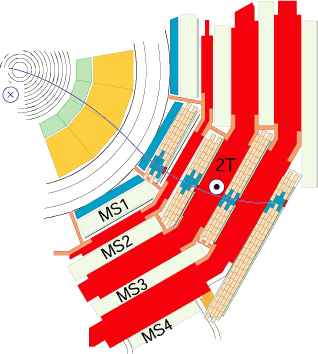
\includegraphics[width = 0.5\linewidth]{images/MuStations.png}
    \caption{Schematic focus representation of the muon system}
    \label{muon_system}
\end{figure}
\subsection{Trigger}
As we previously said, in LHC the beams in the proton interactions cross every 25 ns, and this brings a crossing frequency of 40 MHz. We also stated that multiple interactions happen at the same time.\\
However, the CMS experiment can record only about a thousand events per second.\\
This shows that a severe rate reduction has to take place to store and process data. This is made by the trigger system in two steps, where potentially interesting events are selected and stored for analysis.\\
The \emph{Level-1 trigger} (L1)  brings the rate from 40 MHz to 100 kHz in about 3.8 $\mu$s. It consists of custom-designed electronics that evaluate information from the detector (transverse energies from ECAL and HCAL, tracks isolation, muon trigger), reconstruct some information about the event (like the total transverse energy and the missing energy) and about the particles ($p_T$, $\phi \text{and} \eta$ coordinates), and decide if the event is to be kept or rejected based on the number of jets, thresholds on $p_T$ or $E_T$, and also the topology of the event.\\
The \emph{High Level Trigger} (HLT) brings the rate from 100 kHz to 1 kHz in about 300 ms. It is a software system implemented in a filter farm of about 30,000 commercial cores that further reconstructs the event and looks for more specific event signatures to decide whether to store an event. Because of the time requirements for this analysis, the events are reconstructed in multiple steps and rejected as soon as there is enough information to do so.
\section{Events Reconstruction}
As we introduced, particles of an event are detected by studying the hits left in the different sections of the detector. In principle, one would need only information from the specific subdetector, for example:
\begin{itemize}
    \item jets come from hadrons and photons, and their energy can be reconstructed inclusively without separating individual jet particles. This means that jet reconstruction can be done with the use of HCAL (and ECAL) only, without using information from muon detectors and trackers;
    \item missing transverse momentum and missing transverse energy can be reconstructed with the use of calorimeters only;
    \item isolated photons and electrons need information from ECAL only for reconstruction;
    \item tagging specific particles like $\tau$ leptons and b quarks that have hadronized can be done with information from tracker only;
    \item muons can be identified with information from the muon detectors only.
\end{itemize}
However, a more refined approach, called particle-flow (PF) reconstruction, allows a significant improvement in the description of an event. A brief summary of this approach follows, while a more comprehensive description can be found at Ref. \cite{particle_flow}.\\
In the PF approach, the basic elements from all subdetectors are used to identify each particle in the final state.
\subsubsection{Charged-particle tracks and vertices}
The first important element is the track reconstruction. For this, a combinatorial track finder based on Kalman Filtering (cit) is used to reconstruct the charged-particle trajectory and its properties: transverse momentum, origin, and direction. A track is accepted if it has at least a number of hits inside the tracker, and if it originates within a cylinder of a few mm of radius centred around the beam axis. 
\section{HL-LHC Upgrade}
\label{sec:HL-LHC}
To extend the sensitivity for new physics searches, a major upgrade of the LHC was decided, called the High Luminosity LHC (HL-LHC). With this upgrade, the luminosity of the collider will be greatly enhanced. \\
For this reason, a Long Shutdown (LS3) was planned for 2023. However, because of the COVID-19 pandemic, the LHC was forcefully shut down, and LS3 was postponed to the end of 2024, as can be seen from the schedule in fig. \ref{lhc_schedule}.
\begin{figure}
    \centering
    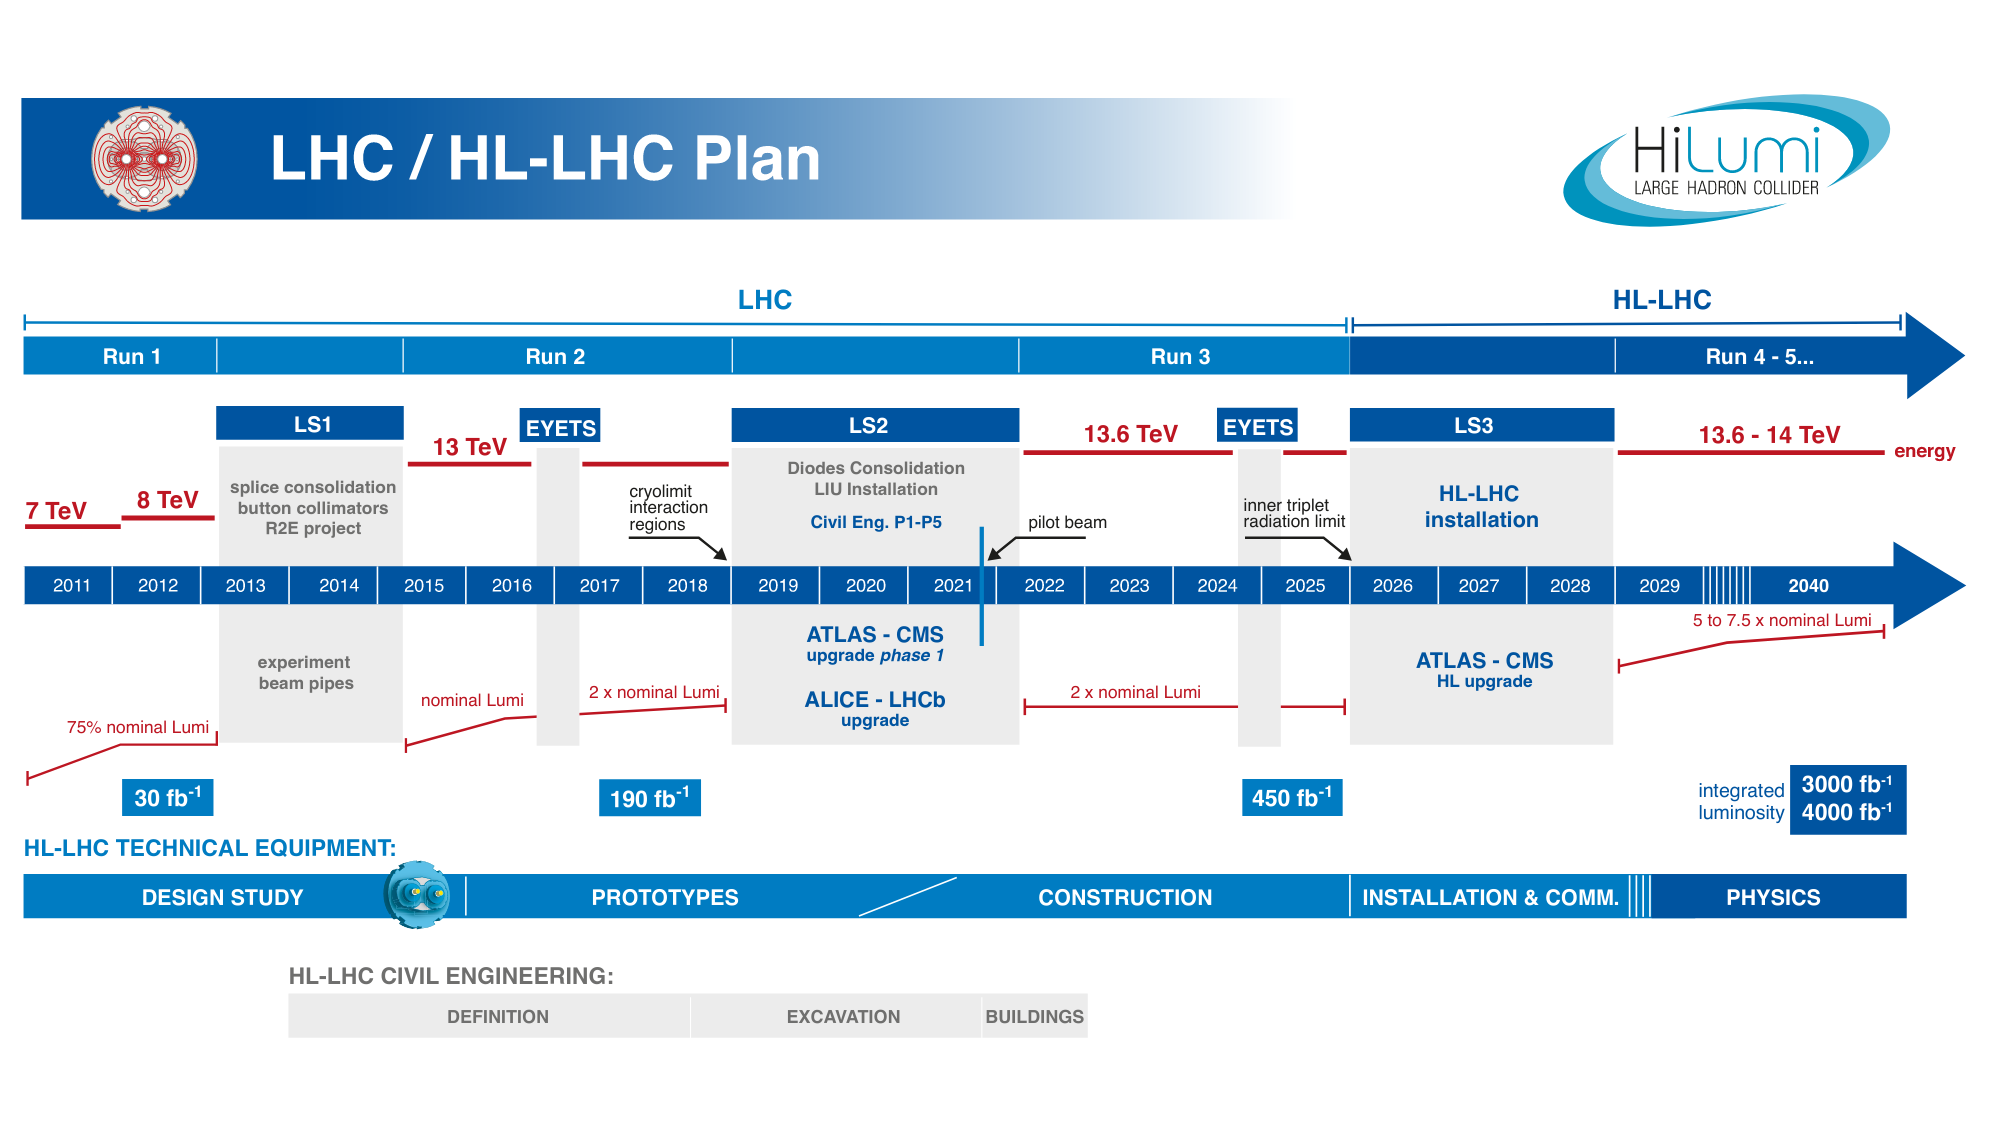
\includegraphics[width = \linewidth]{images/lhc_schedule.png}
    \caption{LHC Schedule considering the forced shutdown due to COVID-19}
    \label{lhc_schedule}
\end{figure}
Fig. \ref{hl_lumi} shows the peak luminosity and the integrated luminosity throughout the years and the expected values for the HL-LHC era.
\begin{figure}
    \centering
    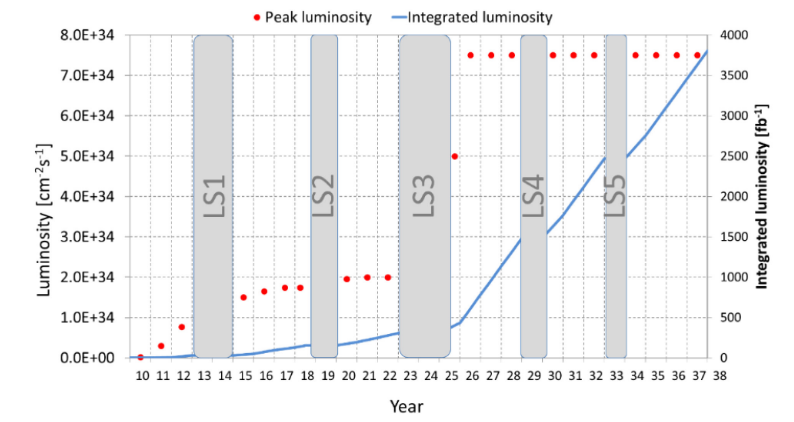
\includegraphics[width = \linewidth]{images/hl_lumi.png}
    \caption{Peak luminosity (red dots) and integrated luminosity (blue line) with the projection of performance of the HL-LHC phase after LS3.}
    \label{hl_lumi}
\end{figure}
The ultimate targets of the project are the following:
\begin{itemize}
    \item Peak luminosity of 7.5 x 10$^{34}cm^{-2}s^{-1}$;
    \item Integrated luminosity of 300-400 fb$^{-1}$ per year, with the goal of 4000 fb$^{-1}$ in the 12 years after the upgrade.
\end{itemize}
These targets require the main experiments ATLAS and CMS to cope with an average pile-up of at least 140, which should increase to 200 in the later period, and obviously increased radiation.
For these reasons, the main equipment modifications will be done in the two major experiment locations, LHC Point 1 (P1 - ATLAS) and LHC Point 5 (P5 - CMS).\\
\subsection{Upgrades to the experiment}
Some of the most relevant upgrades to the CMS detector are listed. The complete upgrade project is reported in Ref. \cite{phase2_tdr}.\\
\begin{itemize}
    \item The silicon tracker must be replaced because of the radiation damage it will sustain by the end of Run3. Furthermore, to maintain the resolution of track reconstruction at high pileup, the granularity of both the inner pixel tracker and the outer tracker needs to be increased. This will improve the $p_T$ resolution, decreasing the trigger rate at a given transverse momentum.
    \item To have a more efficient trigger at low $p_T$ (in particular for $p_T\geq 2$GeV), a new approach will be adopted, that is, the addition of tracking information at L1. This leads to the necessity of new hardware to incorporate the tracking information. 
    \item The endcap calorimeters will also suffer significant radiation damage. The replacement planned is called High Granularity Calorimeter (HGCAL), and will have both the electromagnetic and the hadronic sections. It will consist of a sampling calorimeter with silicon detectors in the inner region, and scintillators in the outer region. Given the granularity of HGCAL, it will also be able to identify tracks and discriminate between charged pions and muons, which, as stated, are present in the forward region. The electromagnetic section will consist of tungsten and copper plates interleaved with silicon scintillators; its width will be 25$X_0$ and 1 $\lambda$. The hadronic section will have a front section of bass and copper plates interleaved with silicon sensors for a width of 3.5$\lambda$, and a "backing hadron calorimeter" similar to HE, with brass plates interleaved with plastic scintillating tiles to provide an overall depth of $\approx10\lambda$ for the full calorimeter.
    \item For CMS in particular, it is of vital importance to improve the resolution of muon detection, especially in the forward region, and this will be done by adding muon chambers and muon detectors, so that a more precise measurement of $p_T$ at L1 level will keep a manageable trigger rate without having to increase the threshold, and so risking to potentially lose new physics at low $p_T$.
    \item Furthermore, Phase-2 will see extended coverage of the inner tracker up to $|\eta|=4$, and this upgrade must be matched with an extension of the muon detection system in the very forward region as well, because the tracker alone cannot identify muons. For this reason, the muon system will be expanded up to $|\eta| \approx 3$. The increase in acceptance in this region is very useful, for example in studying multi-lepton final states like the golden channel.
    \item Latency for L1 was limited to 3.4 $\mu$s by the tracker readout. In Phase-2, it will be increased to 12.5 $\mu$s to provide sufficient time for the hardware track reconstruction and the matching of tracks from the muon system and the calorimeters. With the upgrades, the trigger acceptance rate will be 500 kHz for a PU of 140.
\end{itemize}
\subsection{Physics program}
Thanks to the upgrade, the available dataset after the end of the HL-LHC era will be ten times larger than the one available now. This means that processes with very low cross-section and/or decay branching fractions might be visible.\\
Starting with the Higgs boson, HL-LHC will permit the measurement of the Higgs trilinear self-coupling, and subsequently the study of the Higgs potential. Furthermore, a more detailed study of the properties of the Higgs boson will be possible, for example, the CP, the total width, and the measurement of very rare decay channels.\\
HL-LHC will also allow the search for a more extended Higgs sector, both at higher and lower masses than 125 GeV.\\
All the preliminary studies of the detector performance are made using the Delphes fast simulation \cite{delphes}.\\
A list of some of the objectives for the HL-LHC are reported \cite{HL-LHC_Higgs}, \cite{phase2_tdr}.
\subsubsection{H$\longrightarrow $ZZ$^* \longrightarrow 4 l$}
As previously stated, this is the golden channel in the study of the Higgs boson. Electrons and muons can be measured very accurately, with high efficiency and excellent energy and momentum resolution. This means that the final state can be reconstructed, and this leads to a signal with high purity, which is measured as a peak over a smooth background.\\
This channel is very interesting because studying the angular distributions, like the angle between the ZZ decay planes and the decay angles in these planes, allows a detailed analysis of the CP properties of the Higgs boson and of its total width.\\
The projections of Phase 2 show a significant increase in the selection efficiency after a full selection. 

\subsubsection{H $\bm{\longrightarrow \mu\mu}$}
So far, the only decay modes observed for the Higgs boson have been the ones to the third generation of fermions (\emph{t}, \emph{b}, $\tau$), and with the vector bosons. \\ 
So, an important test to the SM is the study of the Higgs coupling with the fermions of the second generation, which, however, have smaller values and smaller experimental rates.\\
The easier one from the experimental side is the decay of the Higgs boson in two muons, which has a branching fraction expected from the SM of $2.2 x 10^{-4}$. Furthermore, the events can be fully reconstructed, and the signal will appear as a small bump on the di-muon background from Drell-Yan events, and this means that an excellent resolution on the di-muon mass is needed.
\\
Evidence of the Higgs decay in a pair of muons was presented in 2020 with an observed (expected) significance of 3.0 (2.5) standard deviations \cite{H_mumu}.\\
The simulations made of the upgraded Phase-2 tracking detector show an improvement on the mass resolution of 40\%, and an improvement of 20\% on the reconstruction efficiency of the muon pair.
\subsubsection{H $\bm{\longrightarrow \tau \tau}$}
From projections, modifications of the Higgs coupling constant to tau leptons from its SM value can be measured with a precision of 2-5\%, and from BSM Higgs models, modifications comparable or larger to this are to be expected, especially in the hypothesis of multiple Higgs doublets.\\
This makes the H $\longrightarrow \tau \tau$ a good channel to search for new physics.\\
The study of this channel heavily relies on the performance of the whole CMS detector, because the analysis uses electrons, muons, hadronic taus, jets, and missing transverse energy; for this reason, high efficiency and low misidentifications are needed to control the high background. \\
\subsubsection{Higgs boson pair production}
One of the upgrade's main objectives is observing the trilinear coupling of the Higgs boson. This process is also sensitive to BSM physics, which might modify the rate of pair production. Various final states of the Higgs pair will be studied, with their branching fractions are reported in table \ref{pair production BR}:
\begin{itemize}
    \item $\bm{bb\gamma\gamma}$: the signal events contain two high-$p_T$ photons and two high-$p_T$ jets coming from b quarks. For this channel, only 320 events per experiment are expected to be produced with an integrated luminosity of 3 ab$^{-1}$, but it's one of the most sensitive channels to HH production. The background can be mainly divided into two categories: the resonant one and the non-resonant one. The resonant category contains processes like ZH, $t\Bar{t}H$, $b\Bar{b}H$, where the Higgs boson decays in two photons; the non-resonant category contains processes like $b\Bar{b}\gamma\gamma$, $jj\gamma\gamma$, where $j$ are jets from light quarks and are mis-tagged as b jets, or also processes like $b\Bar{b}jj$ or $b\Bar{b}j\gamma$, with one or two jets are misidentifies as photons. The non-resonant backgrounds have cross-sections several times larger than the resonant one, but they are expected to be suppressed by the low rates of misidentification and mis-tagging, also thanks to the improvement that will be obtained on both the parameters (cambiare la parola) during Phase-2.
    \item $\bm{bb\tau\tau}$: for an integrated luminosity of 3 ab$^{-1}$, about 9000 $bb\tau\tau$ events are expected. However, there is an overwhelming contribution of $t\Bar{t}$ background with fully leptonic decays, as well as Drell-Yan production of a Z boson decaying into a pair of tau leptons that are produced with jets coming from light quarks misidentified as b quarks, and single Higgs production, in particular ZH and $t\Bar{t}H$, while QCD multi-jet background is negligible in the signal region. The discrimination of the signal is challenging because of the incomplete reconstruction of the event due to the presence of missing energy from neutrinos of the $\tau$ decays. A cinematic bounding variable is introduced to better discriminate the $t\Bar{t}$ background from the di-Higgs signal. The expected significance for the production in this final state with the combination of $\tau_h \tau_h$ and $\tau_h \tau_{mu}$ is 0.9 standard deviations.\\
    The $\tau \tau$ final state is also interesting for testing BSM physics, for example introducing additional interactions between leptons and hadrons.
    \item $\bm{bbVV}$: both $bbWW$ and $bbZZ$ are considered, even though the most relevant in terms of statistics is the prior. During HL-LHC, about 1800 events are expected from the fully leptonic decay of the W bosons. The dominant background is given by $t\bar{t}$ production with fully leptonic decay. Selected events are required to have two b-tagged jets and two opposite-sign leptons. The results from the preliminary studies suggest a promising contribution of this final state when combined with the other final states that have been considered.
    For the $bbZZ$ decay, 17 events are expected, and they are required to have at least 4 muons or electrons, in addition to the two b-jets coming from the decay of one of the H bosons. The two Z boson candidates are formed from pairs of opposite-charge leptons, with invariant mass around the nominal Z mass; the most relevant background comes from single H production with 4$l$ in the final state.
    \item $\bm{bbbb}$ It has the largest branching fraction, with an expected number of events at the end of HL-LHC of about 37000. However, it is also the channel with the largest QCD multi-jet background. For this reason, the events from this channel are divided into two categories: 
    \begin{itemize}
        \item in the case where the four b-jets can be reconstructed separately the category is called "resolved", and multivariate methods are explored to face the overwhelming background; resolved topology corresponds to the large majority of SM events. In the analysis, the four selected b-jets are combined into two Higgs candidates, H$_1$ and H$_2$ so that the invariant mass is minimal. Because of the large QCD background, a multivariate variable is defined using a Boosted Decision Tree (BDT) to identify the HH signal contribution, and it is used as a discriminator variable
        \item in the case where the invariant mass of the HH system is big, it can happen that the two b-jets from the same H decay overlap and are reconstructed as a single, larger jet, and this category is called "boosted". Boosted topology helps the discrimination of the signal from the background, and provides sensitivity to BSM physics as well, in scenarios where the pair production is enhanced at high values of $m_{HH}$, for example with the presence of ttHH and ggHH contact interactions. Algorithms for b-tagging are used on the sub-jets contained inside the b-jets.
    \end{itemize}  
\end{itemize}
\begin{table}[ht]
    \centering
    \begin{tabular}{c|c}
        Channel & BR [\%] \\\hline 
        $bbbb$ & 33.9 \\\hline
        $bb\tau\tau$ & 7.3 \\\hline
        $bbVV$ (FL) & 1.73 \\\hline
        $bb\gamma\gamma$ & 0.26 \\\hline
    \end{tabular}
    \caption{Branching ratios for the dominant channels of pair production. For the gauge bosons, only the fully leptonic (FL) decay is considered}
    \label{pair production BR}
\end{table}

The different channels are combined statistically, assuming SM Higgs branching fractions. Assuming the presence of a SM signal, the total expected significance is 2.6 $\sigma$; on the contrary, in the background only hypothesis, the expected upper limit on the SM pair production cross-section can be set to 0.77 times the SM prediction.\\
Prospects for the study of the H self-coupling are studied. In the hypothesis of SM HH signal exists, the following confidence intervals can be set:
\begin{equation}
    \kappa_{\lambda} = [0.35, 1.9] \quad 68 \% \text{CL}
\end{equation}
\begin{equation}
    \kappa_{\lambda} = [-0.18, 3.6] \quad 95 \% \text{CL};
\end{equation}
in the hypothesis of background only, upper limits on the HH SM cross-section are derived as a function of $\kappa_{\lambda}$.\\
The results expected are reported in fig. \ref{prospect_HH}.

\begin{figure}
    \centering
    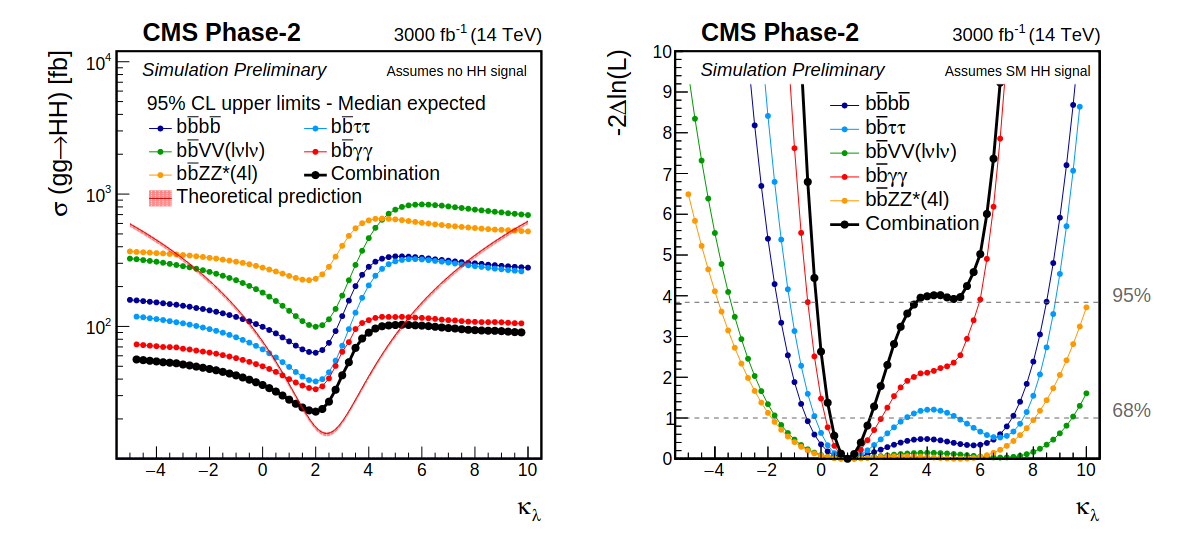
\includegraphics[width =\linewidth]{images/prospects_HH.png}
    \caption{Left: upper limit at 95\% CL on the HH production cross-section as a function of $\kappa_{\lambda}$; the red line shows the theoretical production cross-section. Right: expected likelihood scan as a function of $\kappa_{\lambda}$}
    \label{prospect_HH}
\end{figure}
\subsubsection{Vector Boson Scattering}
Vector Boson Scattering (VBS) is a powerful tool for investigating new physics, because of the high sensitivity to the electroweak symmetry breaking.\\
In particular, the Higgs field not only gives mass to the vector bosons, but also unitarizes the scattering amplitudes of longitudinally polarized bosons, by providing them with the longitudinal degrees of freedom needed to prevent the theory from diverging at high energies.\\
If SM is an effective theory with an additionally strongly-coupled sector, the unitarization of the VBS wouldn't come from the Higgs boson only, but from this new sector as well, which would appear at high energy scales.\\
For this reason, the observation of VBS would help in probing these scales.\\
At HL-LHC the VBS will be accessible when two quarks from the beam protons emit vector bosons, which then interact with each other. The two quarks deflecting will create jets that can be tagged to identify this category of events.\\ 
An example of event is shown in fig. \ref{vbs}
\begin{figure}[ht]
    \centering
    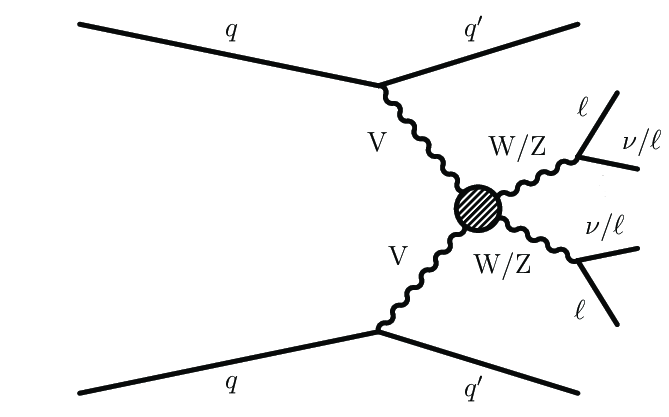
\includegraphics[width=0.4\linewidth]{images/vbs.png}
    \caption{Feynman diagram that shows an example of VBS with fully leptonic final state}
    \label{vbs}
\end{figure}
However, this category of events has a small cross section and suffers from the presence of a very high irreducible background, that is, the production of vector bosons and hadronic jets via strong interactions, to which the misidentification of jets-leptons has to be added.\\
For these reasons, the improvements from the upgrade will be beneficial, in particular the improvement on the jet-lepton misidentification, the extension in coverage of the tracking system up to $|\eta| = 4$ and the highly granular forward calorimeter, which will help with the contamination from jets coming from pileup.

\subsubsection{Other searches}
Studies on B physics are expected to be feasible, in particular in the case of rare processes like $B^0_{(s)}\longrightarrow \mu^+ \mu^-$ decays.\\
Furthermore, other sectors of SM and BSM are expected to be probed, for example, further studies on particles predicted from the SUSY framework, exotica searches, such as different SM extensions, dark matter, and new particles related to mechanisms that might give mass to the light neutrinos.\\

